% !TeX program = xelatex
% Written from the experimental evidence as a standalone English manuscript.
% Compile from the repository root, or upload the accompanying Overleaf ZIP.
\documentclass[aps,prd,12pt,twocolumn,superscriptaddress,floatfix]{revtex4-2}

% REVTeX 4.2 needs the legacy array interface on recent TeX Live releases.
\usepackage{array}[=2016-10-06]
\usepackage{amsmath}
\usepackage{booktabs,tabularx}
\usepackage{graphicx}
\usepackage[a4paper,margin=0.7in]{geometry}
\usepackage[protrusion=true,expansion=false]{microtype}
\usepackage{xurl}
\usepackage[hidelinks,breaklinks=true]{hyperref}
\graphicspath{{artifacts/figures/d7_paper_evidence/20261117_final/}{./}}
\setlength{\emergencystretch}{2em}
\raggedbottom

\begin{document}

\title{Candidate Quality and Logical-Transition Selection in Neural Pre-Decoding for Surface Codes}
\author{Jaemin Jeon}
\affiliation{Korea University}
\date{November 18, 2026}

\begin{abstract}
A neural pre-decoder can propose a useful syndrome modification and still reduce decoding accuracy by applying it to the wrong shot. We study this distinction by comparing the original and modified PyMatching predictions on the same simulated surface-code records. At distance seven under strong ZZ noise, the highest-scoring candidate repaired 10,501 erroneous model--shot predictions but damaged 25,126 correct ones. An oracle restricted to the same edited shots recovered 25,131 additional correct predictions, of which 25,126 simply preserved the original correct answer. A separate candidate-generator control showed that, with 32 nonzero candidates, learned generation covered 88.70\% of original errors versus 77.63\% for local enumeration, a difference of 11.07 percentage points with a 95\% map-level interval of [7.63, 14.51]. This candidate advantage did not establish a gain for the evaluated selection policies. On independent strong-ZZ maps, the frozen margin policy changed accuracy by \(-0.035\) percentage points relative to PyMatching, with a 97.5\% interval of [\(-0.082\), \(+0.013\)]. A gate before candidate generation reduced the existing selection policy's batch time, while its accuracy gain remained uncertain. Finally, we redistributed data-qubit Pauli noise at fixed total channel probability and used bias-matched PyMatching as the reference. At bias \(\eta=20\), independent gains were \(+0.004\) percentage points for the existing margin and \(+0.018\) for a linear selection model retrained on biased data, with both 95\% intervals including zero. These experiments identify candidate selection as the unresolved step in this implementation and distinguish candidate coverage from a demonstrated decoding improvement.
\end{abstract}

\maketitle

\section{Introduction}

Surface-code decoding infers logical errors from repeated local stabilizer measurements \cite{fowler2012}. A decoder must interpret both the observed detection events and the physical noise assumptions used to assign their probabilities. PyMatching provides a fast minimum-weight perfect matching (MWPM) baseline for this task \cite{higgott2022,sparseblossom2025}.

A pre-decoder introduces another decision. After observing a syndrome, it may modify a small subset of detector bits and ask the global decoder to decode the modified record. Such a modification can recover a logical answer that the original decoder missed. It can also overturn a correct answer. Average accuracy alone does not reveal whether a failure arose because no useful modification was proposed, because the available modifications were ranked poorly, or because an unnecessary logical transition was accepted.

This study follows each shot through both the original and modified decoding paths. We ask whether learned candidates contain correct logical answers more often than a simple local rule, whether a policy can select those answers without access to truth, and whether screening shots before candidate generation offers a useful accuracy--cost tradeoff. We then test transfer and selection-model retraining under Pauli-biased noise, using a decoder whose weights already reflect that bias.

Neural local pre-decoding combined with a global decoder has been demonstrated previously \cite{chamberland2026}. Here, a detector edit is a hypothesis used to probe the downstream logical decision. We do not assign each edit a demonstrated physical-error correction and its associated logical parity. The contribution is an evaluation that tracks candidate availability, ranking, and acceptance on identical shots, with explicit counts of repairs and harms and independent evaluation after policy selection.

Decoder confidence and noise-model compatibility motivate several of our controls. Complementary matching costs have been used to convey logical confidence in yoked surface codes \cite{yoked2025}, and decoder switching uses reliability information to allocate decoding effort \cite{toshio2025}. Studies of local-noise adaptation and drifting-noise confidence show why these quantities should be assessed with the assumed decoder model made explicit \cite{darmawan2024,hoyt2026}. We therefore examine class-constrained matching costs and cross decoder priors, while distinguishing a change in the baseline from an additional benefit of pre-decoding.

The results support a limited conclusion. The learned generator outperforms the tested enumeration rule in correct-candidate coverage at the same candidate budget. However, the frozen policies examined here do not establish additional accuracy on the primary independent distance-seven comparisons. The fixed-total Pauli-bias follow-ups reach the same statistical conclusion for the existing margin and the newly fitted linear selection model. These findings delimit what this implementation has achieved and what remains unresolved.

\section{Experimental framework}
\label{sec:framework}

\subsection{Circuit, observables, and noise}

Stim generates samples from rotated surface-code Bell-pair Z-readout circuits \cite{stim2021}. In the main experiments, the code distance and the number of syndrome measurement rounds are both 7. Each shot has two logical-flip bits, ordered as \([Z\text{ flip},X\text{ flip}]\). Truth \((z,x)\) has class index \(2z+x\). Both bits must agree with truth for a prediction to count as correct. The logical error rate is the fraction of shots with at least one incorrect logical bit.

A local noise map specifies physical error probabilities at circuit locations. With reference physical error rate 0.0015, we compare weak ZZ noise \(G_0\), with ZZ coefficient 0.05, and strong ZZ noise \(G_1\), with coefficient 0.25. They share the ideal circuit and local map, use separate sampler seeds, and retain the same base-noise and swap terms. Increasing the ZZ coefficient also changes the total error load. This experiment therefore does not isolate noise composition at fixed total probability.

The detector error models (DEMs) obtained from \(G_0\) and \(G_1\) are denoted \(D_0\) and \(D_1\). We consider ordinary MWPM and correlated PyMatching with each DEM. The predeclared primary strong-ZZ evaluation uses \(G_1\) samples decoded with \(D_0\) ordinary MWPM. Other decoder cells provide prior and matching-mode controls.

A separate experiment changes the Pauli composition of data-qubit single-qubit gate and idle channels. It uses ZZ coefficient 0.05 and swap coefficient 0.02. At an affected location, the original total error probability \(q\) is retained and redistributed as
\begin{equation}
\begin{aligned}
\eta&=\frac{p_Z}{p_X+p_Y},\\
p_X=p_Y&=\frac{q}{2(1+\eta)},\\
p_Z&=\frac{q\eta}{1+\eta}.
\end{aligned}
\label{eq:data-pauli-bias}
\end{equation}
The values \(\eta=0.5,5,20\) include the original uniform single-qubit channel and two increasingly Z-biased channels. Measurement, reset, ancilla single-qubit, two-qubit depolarizing, ZZ, and swap probabilities remain those of the same local map. Thus, \(\eta\) describes the changed data-qubit channels, while the complete circuit still contains other noise sources. DEM construction uses the \texttt{approximate\_disjoint\_errors} approximation.

\subsection{Candidate generation and logical transitions}

The neural input is a 36-channel space--time volume containing detector events, check locations and types, and circuit and noise context. A three-dimensional residual trunk produces per-detector edit scores and shot features. Local motifs obtained from training data are placed on the detector lattice, and the detector scores restrict the candidate set. The final distance-seven evaluations allow 32 nonzero binary masks and one no-edit option for each model and shot.

For detector record \(s\), mask \(m\), and downstream decoder \(D\), define
\begin{equation}
y_0=D(s),\qquad y_m=D(s\oplus m).
\label{eq:edited-prediction}
\end{equation}
The transition is the bitwise XOR of \(y_0\) and \(y_m\). A Z transition changes only the first logical bit. The candidate selector combines shot features, edit size, detector geometry and local events, and the downstream logical transition. Candidate benefits and harms are labeled using downstream logical correctness, independent of exact detector-mask agreement.

Figure~\ref{fig:same-shot-method} shows the comparison. Truth supplies training targets and evaluation counts. Inference uses the syndrome, available context, and model and decoder outputs.

\begin{figure*}[tb]
\centering
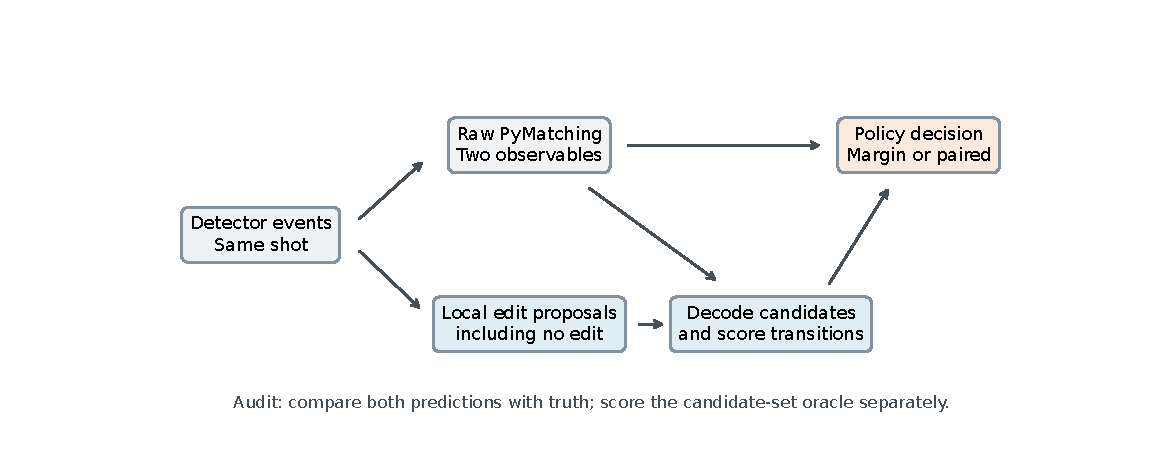
\includegraphics[width=.82\textwidth]{fig01_same_shot_method.pdf}
\caption{Original and edited decoding paths for the same shot. A candidate mask changes the detector record presented to PyMatching. The selector observes syndrome and decoder information. Ground truth is used for training and evaluation.}
\label{fig:same-shot-method}
\end{figure*}

\subsection{Decisions, repairs, and oracle bounds}

Top-1 selects the highest-scoring candidate, including no edit. The per-shot margin retains the original prediction when a nonzero candidate does not clear its checkpoint-specific utility margin over no edit. A separate family gate can disable the edit route for an entire model--noise setting based on development repairs and harms. We distinguish this global decision from shot-level acceptance. The final margin and paired-policy comparison runs without the family gate.

For any policy, a repair changes an incorrect original answer to the correct answer. A harm changes a correct original answer to an incorrect one. If \(R\) and \(H\) are their counts among \(N\) paired predictions, the accuracy difference in percentage points is
\begin{equation}
\Delta_{\mathrm{acc}}=100\,\frac{R-H}{N}.
\label{eq:net-gain}
\end{equation}
Positive values denote a reduction in logical error rate. A changed prediction can also remain incorrect, so the number of changes need not equal \(R+H\).

We use two truth-informed diagnostics. The full candidate oracle counts a shot as correct when at least one candidate, including no edit, predicts its true class. The fixed-shot oracle keeps the policy's edited-shot set and reselects only among nonzero candidates on those shots. It retains the original output elsewhere. The fixed-shot oracle diagnoses ranking losses on the selected shots. The additional gain of the full oracle measures opportunities outside that edited-shot set. Both are upper bounds that require truth and cannot be implemented as inference policies.

\subsection{Input correction and independent evaluation}

An input audit found a context channel containing dataset-level aggregates of the logical labels. We removed this source of evaluation-label information by fixing that channel to zero while retaining the tensor width. The distance-specific models used for all quantitative results reported here were retrained with the corrected input.

Base-model training uses the existing Stage A/B data. Each stage contains 1,024 shots, split into 717 for training, 154 for validation, and 153 for internal testing. Evaluation passes zeros in truth fields when it reuses data structures designed for training.

In later distance-seven experiments, the detector-event fraction supplied as input is fixed at 0.042737, estimated from weak-ZZ development data. Comparisons across decoder priors retain the reference \(G_0\) setting. Final evaluation uses the \(G_0\) context for each map.

Some historical distance-seven family-gate rules were chosen after viewing earlier Stage C outcomes. We therefore freeze subsequent policies and checkpoints before generating new evaluation maps. Table~\ref{tab:map-panels} records the distinct map roles. In particular, maps 788200--788223 first evaluate candidate generators and subsequently serve as development data for the strong-ZZ selection model and gate. Their final evaluations use different, untouched map panels. The first independent biased panel is also excluded from subsequent biased-model fitting and threshold selection.

\begin{table*}[tb]
\centering
\caption{Data panels and fixed model panels. Shot counts are per checkpoint. Reuse of the candidate-comparison panel as later development data is explicit in the text.}
\label{tab:map-panels}
\small
\begin{tabularx}{\textwidth}{@{}>{\raggedright\arraybackslash}X l >{\raggedright\arraybackslash}X l@{}}
\toprule
Purpose & Maps or map IDs & Shots & Checkpoints \\
\midrule
Corrected-input distance validation & 8 per distance & 49,152 at d3 and d5, 32,768 at d7 & Seeds 0--7 \\
d7 noise and transition diagnosis & 8 & 43,008 per ZZ strength & Seeds 2, 11, 54, 57 \\
d7 selector development and calibration & 4 development, 2 calibration & 1,024 per map and strength & Seeds 0--7 \\
Frozen margin evaluation & 788100--788123 & \(G_0\) 6,144; \(G_1\) 12,288 & Seeds 0--7 \\
Candidate-generator comparison & 788200--788223 & \(G_1\) 12,288 & Seeds 0--7 \\
Strong-ZZ selection-model evaluation & 788300--788323 & \(G_1\) 12,288 & Seeds 0--7 \\
Gate evaluation & 788400--788423 & \(G_1\) 12,288 & Seeds 0--7 \\
Pauli-bias pilot & 788500--788507 & Per bias, 65,536 baseline; 16,384 margin & CNN seed 2 \\
Biased margin evaluation & 788600--788623 & \(\eta=20\), 49,152 & CNN seed 2 \\
Biased selection-model training & 788700--788731 & \(\eta=20\), 65,536 & CNN seed 2 \\
Biased threshold selection & 788740--788747 & \(\eta=20\), 16,384 & CNN seed 2 \\
Retrained biased-model evaluation & 788800--788823 & \(\eta=20\), 49,152 & CNN seed 2 \\
\bottomrule
\end{tabularx}
\end{table*}

The eight checkpoints in the main final comparison share the same shots. We average them equally within a map, then average the 24 maps equally. Map-level differences, rather than model--shot pairs treated as independent samples, enter the Student \(t\) intervals. The two primary frozen-margin contrasts each use a two-sided 97.5\% interval. Later gate and biased primary comparisons use two-sided 95\% map-level intervals. We report their confidence levels separately. An interval containing zero leaves the direction of improvement inconclusive.

These intervals describe variation across new local noise maps conditional on the fixed trained models. They do not incorporate variation from new training runs. Biased follow-ups use one fixed candidate CNN, so shot counts and model--shot counts coincide.

\section{From candidate availability to selection failure}
\label{sec:diagnosis}

\subsection{Distance validation and the hidden edit route}

Corrected-input revalidation gives different outcomes at the three distances (Table~\ref{tab:distance}). At distance three, all eight checkpoints adopt the edit route and the policy gains \(+2.260\) pp. The \(+0.022\) pp gain at distance five comes from one adopting checkpoint. At distance seven, every family gate returns the original decoder output. Its zero difference and zero-width interval describe identical predictions. They provide no test of the candidate selector operating without that bypass.

\begin{table*}[tb]
\centering
\caption{Independent distance validation after input correction. Adoption is the number of checkpoints using the edit route. Intervals are 97.5\% at distances three and five and descriptive 95\% at distance seven. Accuracy differences are computed before rounding the displayed accuracies.}
\label{tab:distance}
\small
\begin{tabularx}{\textwidth}{@{}lrr>{\raggedright\arraybackslash}Xr@{}}
\toprule
Distance & Raw accuracy (\%) & Policy accuracy (\%) & Accuracy difference and interval (pp) & Adoption \\
\midrule
3 & 92.910 & 95.169 & +2.260 [1.688, 2.832] & 8/8 \\
5 & 90.513 & 90.535 & +0.022 [0.004, 0.040] & 1/8 \\
7 & 87.543 & 87.543 & 0.000 [0.000, 0.000] & 0/8 \\
\bottomrule
\end{tabularx}
\end{table*}

We expose that route on eight distance-seven diagnostic maps, with four checkpoints sharing 43,008 shots per ZZ strength. Under strong ZZ and \(D_0\) ordinary MWPM, top-1 makes 10,501 repairs and 25,126 harms, giving \(-8.501\) pp relative to the original decoder. Every harmed pair has another nonzero candidate that preserves the correct original answer.

The fixed-shot oracle changes this result to \(+6.107\) pp relative to the original decoder. Of its 25,131 additional correct pairs over top-1, 25,126 preserve an originally correct prediction and only 5 repair another original error. The main observed ranking loss is therefore the acceptance of harmful logical transitions on shots that PyMatching already decoded correctly. Allowing oracle reselection across all shots increases the raw-relative gain to \(+11.543\) pp.

The margin policy reduces the strong-ZZ edit rate from 20.72\% to 1.19\%, but its 948 repairs and 1,104 harms still give \(-0.091\) pp. All four family gates then disable editing. Figure~\ref{fig:failure} separates these stages.

\begin{figure*}[tb]
\centering
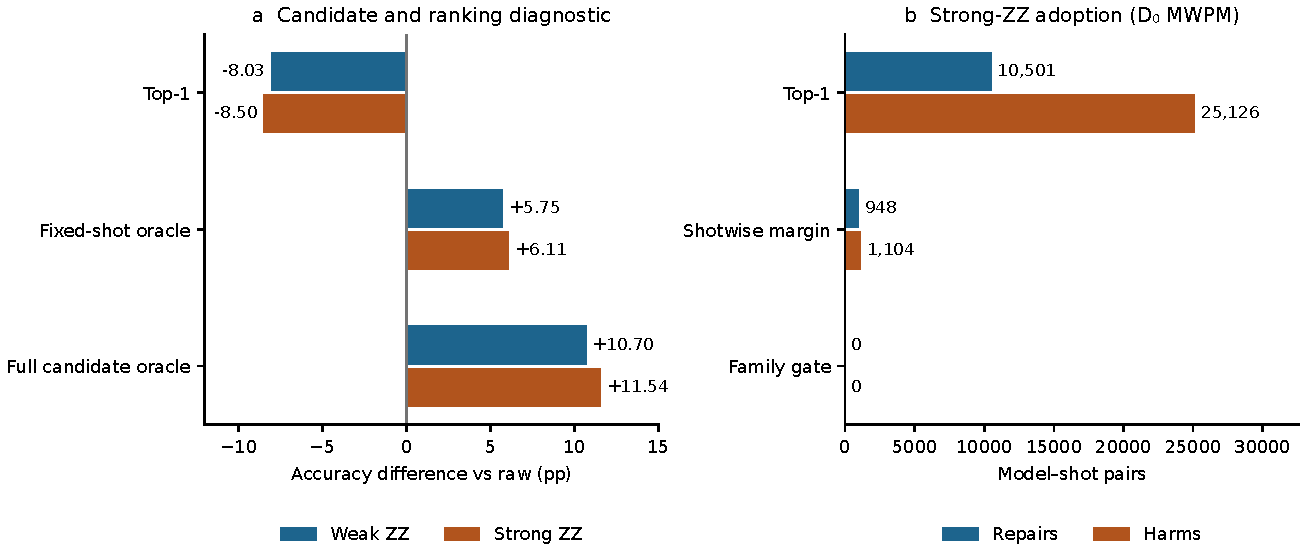
\includegraphics[width=.88\textwidth]{fig02_failure_diagnostic.pdf}
\caption{Candidate-ranking and acceptance diagnosis at distance seven. Left, differences from the original \(D_0\) ordinary-MWPM accuracy. Right, repairs and harms under strong ZZ. The four checkpoints share the same 43,008 shots at each strength.}
\label{fig:failure}
\end{figure*}

The weak-ZZ oracle--top-1 gap is 18.731 pp, and the strong-ZZ gap is larger. However, the predeclared strong-minus-weak difference in top-1 net gain is \(-0.469\) pp with a 97.5\% interval of [\(-0.939\), \(+0.065\)] pp. Together with the changing total error load, this uncertainty limits claims that ZZ strength itself causes the selection failure. We establish the failure pattern in the strong-ZZ setting.

\subsection{Do learned candidates outperform local enumeration?}
\label{sec:candidate-control}

A high oracle score can result from offering several logical answers for a shot. We therefore compare the learned generator with a rule that enumerates active-detector single-bit edits and local pairs containing an active detector. Both receive identical shots, use the same \(D_0\) ordinary-MWPM decoder, and allow one no-edit option plus at most 32 unique nonzero masks. A Manhattan radius of 2 is selected for enumeration on separate development maps.

The primary coverage metric is the fraction of original errors for which at least one candidate gives the true logical class. Maps 788200--788223 contain 12,288 shots and 1,658 original decoder errors. Learned checkpoints are weighted equally within each map, followed by equal map weighting for both generators.

\begin{table*}[tb]
\centering
\caption{Candidate-generator control on 24 new strong-ZZ maps. Coverage is measured among original decoder errors. Only the budget-32 difference is the primary inferential comparison. Smaller budgets are descriptive. The final columns give the mean number of distinct logical classes per shot.}
\label{tab:candidate-control}
\small
\begin{tabularx}{\textwidth}{@{}r rr >{\raggedright\arraybackslash}X rr@{}}
\toprule
\shortstack{Nonzero\\budget} & \shortstack{Learned\\coverage (\%)} & \shortstack{Local\\coverage (\%)} & Coverage difference (pp) & \shortstack{Learned\\classes} & \shortstack{Local\\classes} \\
\midrule
4 & 15.21 & 13.51 & +1.70 & 1.09 & 1.59 \\
8 & 30.75 & 27.79 & +2.97 & 1.20 & 2.00 \\
16 & 58.51 & 51.63 & +6.88 & 1.69 & 2.47 \\
32 & 88.70 & 77.63 & +11.07 [7.63, 14.51] & 2.47 & 2.93 \\
\bottomrule
\end{tabularx}
\end{table*}

At budget 32, learned generation has higher coverage on 22 of the 24 maps. Its mean advantage is \(+11.07\) pp with a 95\% interval of [\( +7.63\), \(+14.51\)] pp (Table~\ref{tab:candidate-control}). Oracle accuracies are 98.449\% and 96.997\% for learned and local generation. All four logical classes appear on 21.16\% and 30.41\% of pairs, respectively. The learned coverage advantage occurs with fewer distinct classes on average.

Candidate quality comes at a computational cost. Median mask-generation times for a 512-shot CPU batch are 1,198.8 ms for learned generation and 96.0 ms for enumeration. Learned timing includes input construction and CNN inference and excludes data and checkpoint loading. These are descriptive measurements from two parallel CPU workers, with 192 learned map--checkpoint batches and 24 local batches. The selection policy is not called in this comparison.

This experiment supports the fixed learned generator over the tested local rule at the same candidate budget. It does not isolate the effect of neural scoring alone. Pattern support, edit weight, and ordering differ jointly. Learned nonzero candidates are all two-bit edits, while 65.9\% of local candidates have weight two, and their spatial supports differ. Candidate availability also remains an oracle property until a truth-free policy can use it.

\section{Selecting logical transitions on independent maps}
\label{sec:selection}

\subsection{Confidence and prior controls}

We first test whether additional downstream confidence can improve selection. The paired-detector policy considers shots whose top-1 candidate changes only the Z bit and that also have a nonzero candidate preserving the original class. It pairs the Z candidate with the highest-scoring original-preserving candidate. A logistic head is fitted on development cases where exactly one of their logical predictions is correct. Its inputs include score differences, geometry, detector patches, the original class, and model identity.

A second set of features uses logical-class matching costs. For a given syndrome, we constrain both observable parities and compute the minimum ordinary-MWPM cost in each logical class. The Z gap compares the current class with the class differing only in its Z bit. We test gaps for both original and edited syndromes, reduced feature sets, a Z-candidate versus no-edit comparison, and original-event-only transition controls. Even the original-based controls require the candidate route to identify the applicable shots.

The constrained costs agree with exhaustive enumeration on small graphs and independent matching calculations on 44 distance-seven syndromes. The largest absolute discrepancy between the constrained-cost and independent calculations is approximately 0.00000117. This number is a solver-validation discrepancy, rather than a difference between logical-class costs.

Cross-validation on the strong-ZZ development maps gives the paired detector an accuracy difference of \(-0.116\) pp from raw PyMatching. Adding the gap changes this to \(-0.095\) pp. The gap improves the paired result by \(+0.021\) pp on average and improves it on three of four maps. Its mean advantage falls below the predeclared \(+0.05\) pp requirement for adopting a more complex configuration.

Both original-based Z controls make no switches under strong ZZ. We retain the existing margin for final evaluation. Its gains are \(+0.012\) pp on development and \(-0.018\) pp on separate calibration maps (Fig.~\ref{fig:development}).

\begin{figure*}[tb]
\centering
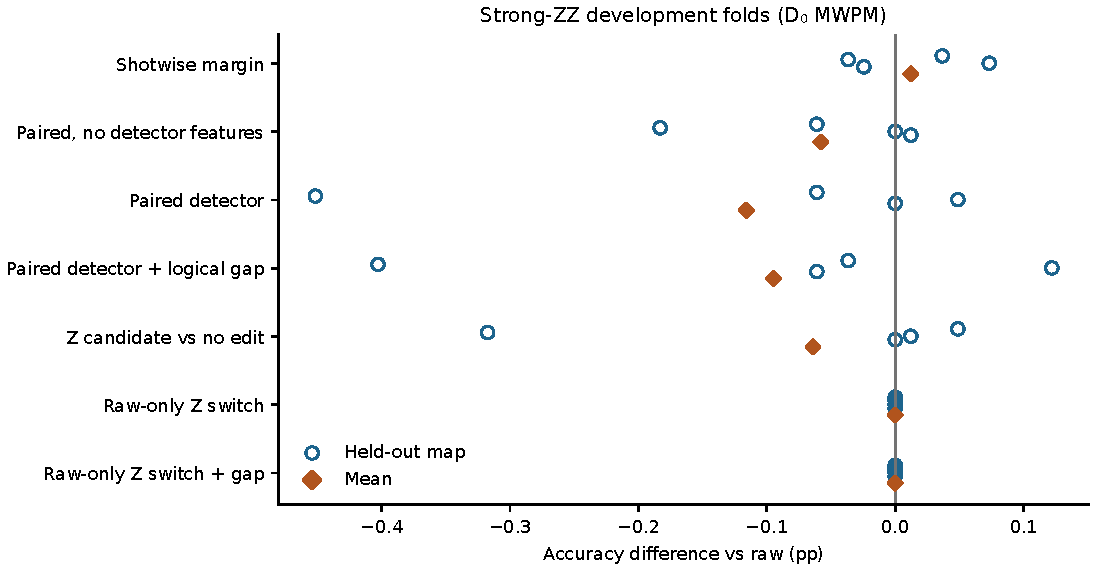
\includegraphics[width=.82\textwidth]{fig03_selector_development.pdf}
\caption{Selection-policy development under strong ZZ. Circles show raw-relative gains on maps held out from head fitting. Diamonds are equally weighted means over the four development maps.}
\label{fig:development}
\end{figure*}

Simpler changes to the scores also fail to establish a useful ranking intervention. Adding the difference between the optimum costs of the original and edited syndromes changes some masks. With the edited shots held fixed, however, the logical outputs remain identical. A constant calibration by original class and transition also leaves candidate choices unchanged on that fixed set. An available feature therefore still needs to demonstrate a benefit through the implemented selection rule.

We also separate decoder-prior effects from selection effects. For the prior comparison, we either keep the masks selected with \(D_0\) ordinary MWPM or recompute logical-transition features and selection using the new decoder. The reference is always the unmodified decoder in the same cell. On the two strong-ZZ calibration maps, raw \(D_1\) correlated matching improves on raw \(D_0\) ordinary MWPM by \(+0.244\) pp. The fixed margin masks give \(-0.031\) pp relative to this improved reference. Recomputing the selection gives \(+0.006\) pp, with 30 changed masks and one additional correct prediction across the full route. This small calibration panel supports only a limited assessment. A DEM matched to the sampling circuit describes the original syndrome distribution, and its suitability after hypothetical detector edits remains a separate question.

\subsection{Frozen margin and paired-policy comparison}
\label{sec:frozen-final}

Before generating maps 788100--788123, we freeze checkpoint seeds 0--7, their margins, the paired head, and the sample size. The strong-ZZ panel contains 12,288 physical shots and 98,304 model--shot pairs. Accuracy is 86.344\% for raw PyMatching, 86.310\% for margin, and 86.318\% for the paired detector.

\begin{table*}[tb]
\centering
\caption{Predeclared primary comparisons on the strong-ZZ \(G_1/D_0\) ordinary-MWPM panel. A repair or harm is relative to the comparator named in the first column. Error rates are shown as comparator / margin.}
\label{tab:primary}
\small
\begin{tabularx}{\textwidth}{@{}lrrr>{\raggedright\arraybackslash}X@{}}
\toprule
Comparison & \shortstack{Accuracy\\difference (pp)} & \shortstack{97.5\% interval\\(pp)} & Repairs / harms & Error rates (\%) \\
\midrule
Margin vs raw & \(-0.035\) & [\(-0.082\), \(+0.013\)] & 139 / 173 & 13.656 / 13.690 \\
Margin vs paired & \(-0.008\) & [\(-0.081\), \(+0.065\)] & 283 / 291 & 13.682 / 13.690 \\
\bottomrule
\end{tabularx}
\end{table*}

Both primary intervals include zero (Table~\ref{tab:primary}). Margin exceeds raw accuracy on seven maps, is lower on sixteen, and ties on one. The full candidate oracle reaches 98.115\% accuracy, a raw-relative advantage of \(+11.771\) pp. Available recovery opportunities therefore persist on new maps, but the evaluated margin does not turn them into an established average gain. Figure~\ref{fig:independent} shows map-level and checkpoint-level variation.

\begin{figure*}[tb]
\centering
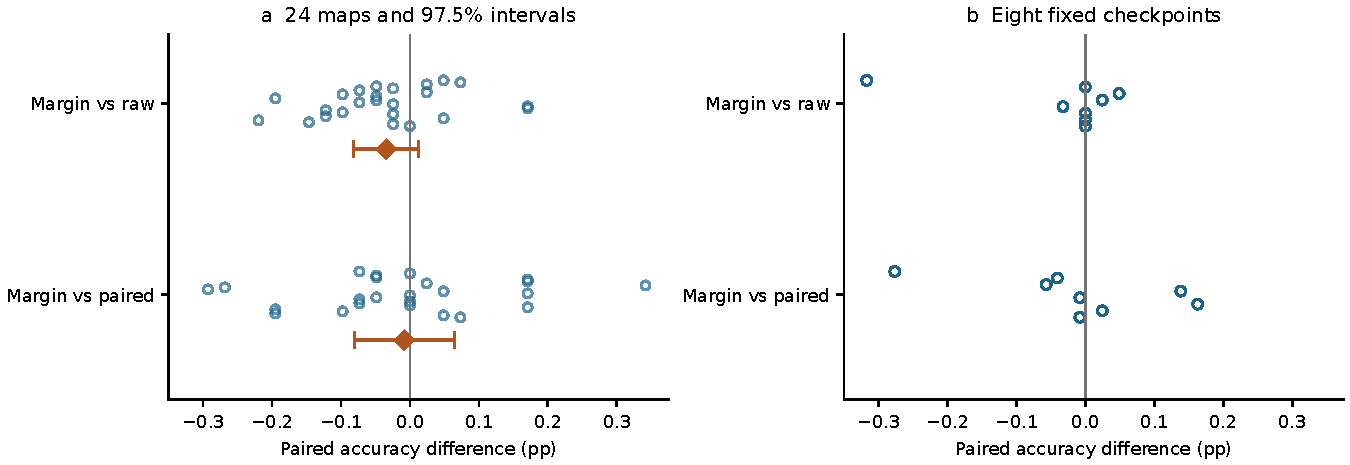
\includegraphics[width=.88\textwidth]{fig04_independent_effects.pdf}
\caption{Independent primary effects. Left, map-level differences and their overall means with 97.5\% intervals. Right, effects for each fixed checkpoint, vertically offset for readability. Shared shots are accounted for by map-level aggregation.}
\label{fig:independent}
\end{figure*}

Secondary comparisons show a \(+0.114\) pp gain for raw \(D_1\) correlated matching over raw \(D_0\) ordinary MWPM under \(G_1\). Adding margin to the former gives \(-0.004\) pp. Paired-policy net gains are positive in all four weak-ZZ decoder cells. These results have different conditions and comparison roles from the primary strong-ZZ analysis and are interpreted descriptively.

\subsection{A class-based selection model}

With the learned candidate set held fixed, we fit a multinomial logistic model to estimate the probabilities of retaining the original class or making an alternative transition. Features include the original syndrome's class-constrained costs and candidate summaries for each logical class. These summaries record counts, first ranks, and cost changes.

The policy compares the highest estimated probability among candidate-supported alternatives with the estimated probability of the original class. It switches only when the difference is strictly greater than 0.025, the threshold fixed during development.

On separate maps 788300--788323, the policy changes 757 model--shot predictions, producing 351 repairs, 401 harms, and five changes that remain wrong. Its raw-relative accuracy difference is \(-0.051\) pp with a 97.5\% interval of [\(-0.199\), \(+0.097\)] pp. Every applied transition is a Z transition. This model changes the decision rule, but the independent evaluation does not establish an improvement.

\section{Computational cost and screening before search}
\label{sec:cost}

\subsection{Cost of the original selection routes}

We benchmark the original raw, margin, and paired routes using checkpoint 2 and the first 256 shots at each ZZ strength from map 788100. Each route runs in a separate process on an Intel Core i7-1165G7, with two PyTorch threads and MKL SEQUENTIAL. We use one warm-up and the median of three repetitions. The measured interval starts with in-memory syndromes and includes input conversion, candidate generation and scoring, and the final prediction. File loading and initial model and DEM preparation are recorded separately.

\begin{table*}[tb]
\centering
\caption{CPU batch costs for 256 shots with \(D_0\) ordinary MWPM. Peak memory is the process working-set maximum during initialization and measurement. Times concern one map and checkpoint.}
\label{tab:cpu}
\small
\begin{tabularx}{\textwidth}{@{}lrrr>{\raggedright\arraybackslash}X@{}}
\toprule
Noise & Raw time & Margin time & Paired time & Peak memory, raw / margin / paired (MiB) \\
\midrule
\(G_0\) & 2.373 ms & 9.173 s & 10.152 s & 268.0 / 346.6 / 350.8 \\
\(G_1\) & 1.635 ms & 12.471 s & 8.246 s & 268.6 / 350.4 / 347.7 \\
\bottomrule
\end{tabularx}
\end{table*}

Raw PyMatching decodes the 256 syndromes in one batch call. Each selection route processes 8,704 rows across 257 calls, with approximately 0.081--0.106 seconds inside matching functions. Candidate construction and neural and candidate scoring account for most elapsed time. Run-to-run variability prevents a firm speed ordering of margin and paired selection. These batch measurements do not measure online latency (Fig.~\ref{fig:cost-accuracy}).

\begin{figure*}[tb]
\centering
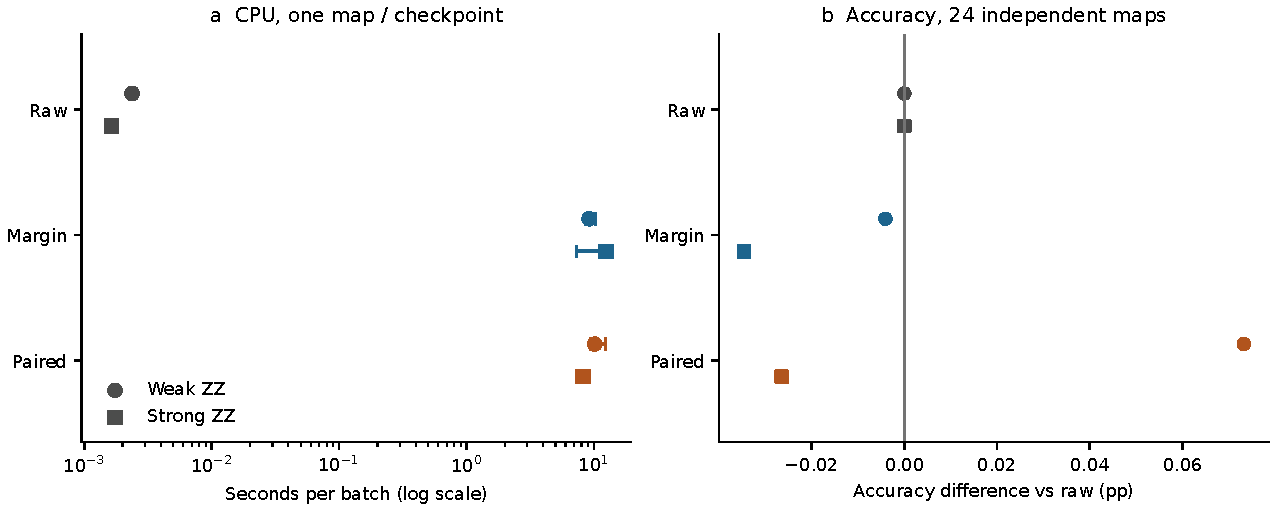
\includegraphics[width=.88\textwidth]{fig05_cost_and_accuracy.pdf}
\caption{Cost and accuracy have different sampling scopes. Left, batch-time medians and repetition ranges for the one-map benchmark. Right, raw-relative accuracy effects over 24 independent maps. Circles and squares denote weak and strong ZZ, respectively.}
\label{fig:cost-accuracy}
\end{figure*}

\subsection{Gate design and frozen adoption criterion}

Candidate search incurs its cost before the policy decides whether to change the logical answer. We therefore fit a gate to decide whether to run that search. The gate uses the cost returned by the first ordinary-MWPM call and detector-event counts for each round. Its training target is \(+1\) for a repair by the fixed downstream selection policy, \(-1\) for a harm, and zero otherwise, averaged across the eight checkpoints. A linear ridge model predicts this target.

A rejected shot retains the original prediction. An admitted shot runs the frozen class-based policy with its strict 0.025 probability-difference threshold. The gate's effect relative to that policy is
\begin{equation}
\Delta_{\mathrm{gate}}=
100\,\frac{\text{blocked harms}-\text{missed repairs}}{N}.
\label{eq:gate-effect}
\end{equation}
Leave-one-map-out development selects the admission threshold by this quantity. Among seven thresholds, a target admission rate of 90\% gives the largest development net count, blocking 45 harms and missing 35 repairs.

Before sampling the final gate panel, we require two conditions for adoption. First, the mean paired batch-time saving relative to the existing selection policy must be positive. For each map this saving is the policy's repetition-median time minus the gated route's repetition-median time. Second, the lower bound of the gated route's 95\% accuracy-difference interval against raw PyMatching must exceed zero. Both conditions must hold.

\subsection{Independent gate evaluation}

On maps 788400--788423, each route receives the same 512-shot batches. Accuracy is evaluated with all eight checkpoints, while timing assigns one checkpoint per map and cycles checkpoints across maps. Route order is rotated over one warm-up and three measured repetitions. The timing covers the first MWPM call, feature and gate computation, any class-cost and candidate work, and the final prediction. Loading and static preparation are excluded for all routes.

\begin{table*}[tb]
\centering
\caption{Gate evaluation on 24 new strong-ZZ maps. Accuracy uses 98,304 model--shot pairs. Intervals are 95\% map-level intervals. Times are medians across maps of repetition-median 512-shot batch times.}
\label{tab:gate}
\small
\begin{tabularx}{\textwidth}{@{}>{\raggedright\arraybackslash}X rrr@{}}
\toprule
Route & \shortstack{Accuracy difference\\from PyMatching (pp)} & Repairs / harms & Batch time \\
\midrule
Raw PyMatching & Reference & 0 / 0 & 3.642 ms \\
Existing selection policy & \(+0.042\) [\(-0.144\), \(+0.227\)] & 418 / 377 & 1.213 s \\
Policy with gate & \(+0.028\) [\(-0.148\), \(+0.205\)] & 350 / 322 & 1.074 s \\
\bottomrule
\end{tabularx}
\end{table*}

The gate runs candidate search on 90.69\% of physical shots. It blocks 55 harms and misses 68 repairs, giving \(-0.013\) pp relative to the existing policy with a 95\% interval of [\(-0.079\), \(+0.052\)] pp. Raw, existing-policy, and gated accuracies are 86.157\%, 86.199\%, and 86.186\%, respectively.

Batch time decreases on all 24 maps. The mean paired saving is 119.1 ms with a 95\% interval of [97.2, 140.9] ms. This mean saving differs from subtracting the two across-map medians in Table~\ref{tab:gate}. Runtime is reduced, and the accuracy gain remains inconclusive. The gate meets the time condition but fails the accuracy condition, so it is not adopted under the frozen rule.

\section{Fixed-total Pauli bias and model readaptation}
\label{sec:bias}

\subsection{Pilot and frozen transfer test}

We also ask whether pre-decoding adds value when the baseline uses a DEM from the actual biased circuit. Equation~\ref{eq:data-pauli-bias} changes the Pauli composition at fixed total probability in each affected channel. The pilot uses eight maps per bias and 8,192 shots per map to compare uniform-channel and bias-matched DEMs with both ordinary and correlated matching. The existing margin runs on the first 2,048 shots of each map.

We select ordinary MWPM because it has the lower error rate on the development data with matched weights. The representative condition is \(\eta=20\), the strongest bias investigated. Candidate CNN seed 2 and its existing selector remain fixed, and we explicitly enable the candidate route.

CNN context retains the pilot's uniform-channel reference metadata and the fixed detector-event fraction. The saved utility margin is 1.25. A nonzero edit is retained when its utility is at least the no-edit utility plus 1.25.

Pilot margin gains over bias-matched PyMatching are \(+0.305\) pp at \(\eta=0.5\), with a 95\% interval of [\( +0.154\), \(+0.456\)] pp, \(+0.128\) pp at \(\eta=5\), with [\(-0.069\), \(+0.326\)] pp, and \(+0.189\) pp at \(\eta=20\), with [\(-0.002\), \(+0.380\)] pp. Changing from the uniform-channel to the biased DEM gives \(-0.044\) pp at \(\eta=5\) and \(-0.037\) pp at \(\eta=20\), with both intervals including zero. These are development results used to choose the follow-up setting.

For the first independent panel, we sample 2,048 shots per map across 24 new maps, giving 49,152 shots in total. The uniform-channel control retains the same local heterogeneity and other circuit-noise terms. The primary comparison evaluates the existing margin against bias-matched ordinary MWPM on the same biased shots.

Margin makes 205 repairs and 203 harms, for \(+0.0041\) pp with a 95\% interval of [\(-0.0859\), \(+0.0940\)] pp. The corresponding error rates are 14.1337\% and 14.1296\% (Table~\ref{tab:bias}). Correct candidates exist for 87.53\% of original errors. Changing the DEM alone produces 45 repairs and 45 harms, a difference of 0.0000 pp with [\(-0.0360\), \(+0.0360\)] pp. Predictions differ on only 90 of 49,152 shots, or 0.183\%.

\begin{table*}[tb]
\centering
\caption{Two independent \(\eta=20\) evaluations, each with 24 new maps and 49,152 shots conditional on candidate CNN seed 2. Policies within a panel share shots. Primary comparisons are existing margin versus bias-matched PyMatching in the first panel and retrained selection versus bias-matched PyMatching in the second. Intervals are 95\% map-level intervals. Positive accuracy differences denote reductions in logical error rate.}
\label{tab:bias}
\small
\begin{tabularx}{\textwidth}{@{}>{\raggedright\arraybackslash}X rrrr l@{}}
\toprule
Policy & \shortstack{Error rate\\(\%)} & Repairs & Harms & \shortstack{Accuracy difference\\from raw (pp)} & 95\% interval (pp) \\
\midrule
\multicolumn{6}{@{}l}{Frozen transfer evaluation, maps 788600--788623} \\
Bias-matched PyMatching & 14.1337 & -- & -- & 0 & -- \\
Existing margin & 14.1296 & 205 & 203 & \(+0.0041\) & [\(-0.0859\), \(+0.0940\)] \\
\midrule
\multicolumn{6}{@{}l}{Evaluation after selection-model retraining, maps 788800--788823} \\
Bias-matched PyMatching & 14.4124 & -- & -- & 0 & -- \\
Existing margin & 14.3778 & 216 & 199 & \(+0.0346\) & [\(-0.0392\), \(+0.1084\)] \\
Retrained selection model & 14.3941 & 199 & 190 & \(+0.0183\) & [\(-0.0702\), \(+0.1068\)] \\
\bottomrule
\end{tabularx}
\end{table*}

\subsection{Selection-model retraining on biased data}

We next retrain the selection model using biased data while keeping the candidate CNN and motifs fixed. The four-class logistic target is the XOR of the original MWPM class and the true class. The 34 input features summarize the original matching cost and class, detector counts by round, class-relative costs and reachability, and the candidate transition counts, first ranks, and edited matching costs. Feature computation receives no truth labels.

The model is fitted on 65,536 shots from 32 new maps. Features are standardized with the training means and standard deviations, using a standard-deviation floor of \(10^{-6}\). The L2 regularization coefficient is 0.01.

Threshold selection uses eight separate development maps with 16,384 shots. The thresholds tested are 0, 0.01, 0.025, 0.05, 0.10, 0.20, 0.35, 0.50, and 1.0. For each shot, the policy considers only the most probable alternative supported by a candidate. Its estimated probability must exceed the probability of retaining the raw prediction by strictly more than the threshold.

We maximize mean map-level development gain, breaking ties toward the higher threshold. Threshold 1.0 always retains the original output. The selected threshold is 0.01, giving 80 development repairs and 63 harms, or \(+0.1038\) pp. A selected transition uses the first candidate producing it in the existing ranking. Retaining the original class uses no edit. The model is not refitted after threshold selection, and coefficient and threshold hashes are saved before independent sampling. This probability threshold and the earlier utility margin of 1.25 apply to different scores.

On 24 further new maps, the retrained model produces 199 repairs and 190 harms, or \(+0.0183\) pp relative to bias-matched PyMatching. Its 95\% interval of [\(-0.0702\), \(+0.1068\)] pp includes zero. The existing margin on these same shots gains \(+0.0346\) pp. New-minus-existing-margin is \(-0.0163\) pp with a secondary 95\% interval of [\(-0.1092\), \(+0.0767\)] pp. Neither comparison establishes an improvement.

Retraining changes the selected shots. The new policy makes 389 logical switches and the existing margin makes 415, all Z transitions. Relative to the margin, the new policy blocks 191 harms, misses 202 repairs, adds 185 repairs, and adds 182 harms. These changes yield eight fewer correct answers overall. Of 7,084 original errors, 6,195 have a correct candidate, corresponding to 87.45\% coverage.

The nominal four-class formulation is highly asymmetric in this setting. Training targets comprise 56,328 original-preserving cases, 10 X transitions, 9,196 Z transitions, and two Y transitions. In the independent panel, 7,077 of the 7,084 original errors, or 99.90\%, could be corrected by changing only the original prediction's Z bit. This experiment therefore primarily tests which shots warrant a Z-bit reversal. The number of output classes alone does not describe the decision problem being tested.

\section{Discussion}

\subsection{Candidate quality and usable accuracy}

The learned generator supplies correct alternatives more often than the tested local rule at budget 32. This is evidence about candidate quality under a fixed downstream decoder. The independent selection evaluations address a different requirement, identifying those alternatives without truth while preserving correct original answers.

The distinction is substantial in the distance-seven diagnosis. Almost all additional correct predictions obtained by the fixed-shot oracle come from preserving an answer that top-1 damaged. On the final margin panel, the actual policy has 34 more harms than repairs even though the full candidate oracle is 11.771 pp above the original decoder. Candidate coverage and the net gain of implemented decisions must therefore be reported together.

A smaller earlier paired-head study reported \(+0.148\) pp over the original decoder on independent strong-ZZ maps with four checkpoints. The later final comparison changes both the fitting data and the fixed model panel to eight checkpoints. Its primary intervals include zero. The earlier positive estimate does not establish a benefit for that later frozen configuration.

\subsection{What the biased experiments resolve}

In the Pauli-bias comparison, each affected data-qubit channel retains its total error probability. Pre-decoding is evaluated against a baseline built from the actual biased circuit's DEM. The independent comparisons of the margin and retrained model both leave additional gains unresolved.

The small effect of changing DEM weights is also informative about this particular setting. Uniform-channel and bias-matched weights produce different logical predictions on only 0.183\% of the first independent panel, with equal repairs and harms. Most predictions remain stable after the weight change. Contributions from unchanged noise channels and stability of matching paths are possible explanations, but their roles have not been established. We restrict the conclusion to the observed prediction-change rate and accuracy difference.

The retrained model learns new coefficients from biased data. Its result applies to a linear decision rule using 34 matching-cost and candidate-summary features, conditional on one fixed candidate CNN. Performance with richer spatial selection features or a candidate CNN trained on biased data remains open. The two independent biased panels contain different maps, so the appropriate assessment of retraining uses the old and new policies on the shared shots of the second panel. Differences between the panels' raw error rates are not estimates of a retraining effect.

\subsection{Runtime and implementation scope}

Screening before candidate generation saves time relative to the existing selection policy. However, search is skipped on only 9.31\% of shots, and the gated 512-shot median of 1.074 seconds remains far above raw PyMatching's 3.642 ms on the same batches. The observed reduction does not establish a practical advantage over the baseline.

The three cost experiments measure different workloads. The original CPU benchmark uses one map and checkpoint with 256-shot batches. The candidate comparison measures generation with two parallel workers. The gate benchmark measures complete routes on the same 512-shot batches across new maps. Timings from these experiments cannot be combined to estimate a route-level speedup. Online latency, latency under biased noise, RTL area, and RTL latency have not been measured.

\subsection{Limits of the evidence}

The evidence comes from simulated Bell-pair circuits evaluated with fixed model panels. Inputs include circuit and noise context derived from simulation. Further evaluation is needed to assess new training seeds, other circuit families, and experimental hardware. Stronger ZZ changes the total error load, while Pauli bias changes only selected single-qubit channels. These experiments do not establish a general result for correlated or biased noise.

Intervals that include zero are compatible with small improvements and small degradations. They do not prove that every pre-decoder or every selection architecture fails. For the evaluated configurations, they do limit claims of an independently reproduced accuracy improvement. The positive distance-three result, the limited distance-five adoption, and the distance-seven bypass should likewise be interpreted separately.

\section{Conclusion}

Following original and edited predictions on identical shots exposes a failure that average accuracy obscures. At distance seven, top-1 predominantly loses accuracy by accepting logical transitions that damage correct PyMatching answers. Learned candidates outperform a simple local enumeration rule in correct-candidate coverage at equal budget, but the evaluated frozen and retrained selection policies do not establish additional accuracy in the primary independent comparisons.

A gate using the first MWPM result and syndrome counts reduces the existing selection policy's CPU batch time. It fails the joint adoption rule because its accuracy advantage over PyMatching remains uncertain. Fixed-total data-qubit Pauli-bias experiments reach an analogous conclusion for both transfer of the existing margin and retraining of a linear selection model. The remaining question for this implementation is how to convert available correct alternatives into a reproducible net gain at acceptable computational cost.

\appendix

\section{Frozen policy details}
\label{app:policies}

Selector development uses four strong-ZZ maps. Each fold fits on three maps and evaluates both strengths on the held-out map. A more complex configuration must exceed its control by at least 0.05 pp on average and on at least three of four maps. After selection, the paired-detector control is refitted on all four strong-ZZ development maps.

For that paired head, the positive label means the Z-transition member of the pair is correct, and the negative label means the original-preserving member is correct. Cases where both or neither are correct are excluded from fitting. Development means and standard deviations transform the features, with a standard-deviation floor of 1. The logistic L2 coefficient is 0.01. A log-odds value of zero or greater selects the Z transition. A negative value retains the original answer. Unpaired shots use the existing margin.

The margins for checkpoint seeds 0--7 are 1.0, 1.0, 1.25, 2.0, 0.5, 1.75, 1.0, and 1.0, respectively. Final evaluation uses maps 788100--788123 and sampler seeds 1794100--1794147. Checkpoint hashes, thresholds, and sample sizes are fixed before generating those data.

Each checkpoint receives 6,144 weak-ZZ shots and 12,288 strong-ZZ shots.

\section{Reproducibility and numerical checks}
\label{app:reproducibility}

% Main evidence: docs/thesis/PREDECODER_PAPER_EVIDENCE.md
% Candidate control: artifacts/eval/d7_candidate_generators/20261117/summary.json
% Selection control: docs/thesis/results/PREDECODER_D7_ADOPTION_RESULTS.md
% Gate: artifacts/eval/d7_pre_gate/20261117/summary.json
% Bias pilot: artifacts/eval/d7_pauli_bias/pilot/pilot_validation.json
% Biased independent evaluation: artifacts/eval/d7_pauli_bias/independent/validation.json
% Biased model retraining: artifacts/eval/d7_pauli_bias_adoption/validation.json

Frozen protocols, source and checkpoint hashes, route predictions, map aggregates, and records for generating figures and tables are retained in the repository. Experiments run with Stim 1.15.0 and PyMatching 2.3.1 in the Anaconda \texttt{fp} environment. The Overleaf package includes the manuscript and five figure PDFs. Experimental datasets and checkpoints are separate research artifacts.

The margin evaluation verifies 384 prediction files and candidate redecoding records for approximately 19,460,000 rows. The 192 files underlying the primary strong-ZZ comparison are independently reaggregated to check repairs, harms, and intervals. Gate validation checks new-map predictions and repeated timings, including agreement with the existing policy on admitted shots.

For biased-model retraining, verification covers 32 training, eight development, and 24 independent maps, including dataset, feature, and prediction hashes. Training normalization and gains at every development threshold are recomputed. Every selected independent-evaluation mask is applied and decoded again. Replacing truth fields leaves inference outputs unchanged. At experiment completion, syntax checks and all 40 tests for the biased follow-up code pass.

We check the affected channels' total probabilities both in memory and in the stored Stim text. The in-memory check uses relative tolerance \(10^{-12}\). Stim text stores six significant digits. In the first independent biased evaluation, the largest absolute sum discrepancy in the stored circuits is \(9.8\times10^{-9}\). The largest relative discrepancy is \(8.29\times10^{-6}\), within the stored-text relative tolerance of \(10^{-5}\).

The biased follow-ups use two parallel CPU workers and include redecoding verification. Their total elapsed times do not measure end-to-end route latency.

\begin{thebibliography}{9}
\raggedright
\bibitem{fowler2012}
A. G. Fowler, M. Mariantoni, J. M. Martinis, and A. N. Cleland, “Surface codes: Towards practical large-scale quantum computation,” Physical Review A 86, 032324 (2012). \url{https://doi.org/10.1103/PhysRevA.86.032324}

\bibitem{higgott2022}
O. Higgott, “PyMatching: A Python package for decoding quantum codes with minimum-weight perfect matching,” ACM Transactions on Quantum Computing 3(3), Article 16 (2022). \url{https://doi.org/10.1145/3505637}

\bibitem{sparseblossom2025}
O. Higgott and C. Gidney, “Sparse blossom: Correcting a million errors per core second with minimum-weight matching,” Quantum 9, 1600 (2025). \url{https://doi.org/10.22331/q-2025-01-20-1600}

\bibitem{chamberland2026}
C. Chamberland, J. Olle, M. Li, S. Thornton, and I. Baratta, “Fast and accurate AI-based pre-decoders for surface codes,” arXiv:2604.12841 (2026). \url{https://arxiv.org/abs/2604.12841}

\bibitem{darmawan2024}
A. S. Darmawan, “Optimal adaptation of surface-code decoders to local noise,” arXiv:2403.08706 (2024). \url{https://arxiv.org/abs/2403.08706}

\bibitem{yoked2025}
C. Gidney, M. Newman, P. Brooks, and C. Jones, “Yoked surface codes,” Nature Communications 16, 4498 (2025). \url{https://doi.org/10.1038/s41467-025-59714-1}

\bibitem{toshio2025}
R. Toshio, K. Kishi, J. Fujisaki, H. Oshima, S. Sato, and K. Fujii, “Decoder switching: Breaking the speed-accuracy tradeoff in real-time quantum error correction,” arXiv:2510.25222 (2025). \url{https://arxiv.org/abs/2510.25222}

\bibitem{hoyt2026}
A. C. Hoyt et al., “Decoder model compatibility provides information beyond the logical gap under drifting and correlated quantum noise,” arXiv:2609.29018 (2026). \url{https://arxiv.org/abs/2609.29018}

\bibitem{stim2021}
C. Gidney, “Stim: A fast stabilizer circuit simulator,” Quantum 5, 497 (2021). \url{https://doi.org/10.22331/q-2021-07-06-497}

\end{thebibliography}

\end{document}
